\documentclass[11pt]{report}
\usepackage[margin=2cm]{geometry}
\usepackage[dvipsnames]{xcolor}
\usepackage{graphicx}
\usepackage{float}
\usepackage{times}
\usepackage[numbers,sort&compress]{natbib}
\PassOptionsToPackage{hyphens}{url}\usepackage{hyperref}
\usepackage{fnpct}

\newcommand{\Gap}{\texorpdfstring{\hfill}{}}
\newcommand{\Rec}{\texorpdfstring{{\small\emph{\color{blue}{\fbox{High Leverage}}}}}{}}
\newcommand{\HighRisk}{\texorpdfstring{{\small\emph{\color{orange}{\fbox{Uncertain Impact}}}}}{}}
\newcommand{\Longterm}{\texorpdfstring{{\small\emph{\color{OliveGreen}{\fbox{Long-term}}}}}{}}

\setcounter{secnumdepth}{3}

\usepackage{color}
\newcommand{\maybe}[1]{{\color{red} #1}}

\begin{document}
\section{Industry\texorpdfstring{\hfill\textit{by Anna Waldman-Brown}}{}}
\label{sec:industry}
Industrial production, logistics, and building materials are leading causes of difficult-to-eliminate GHG emissions \cite{Daviseaas9793}. Fortunately for ML researchers, the global industrial sector spends billions of dollars annually gathering data on factories and supply chains \cite{Gualtieri2016} -- aided by improvements in the cost and accessibility of sensors and other data-gathering mechanisms (such as QR codes and image recognition). The availability of large quantities of data, combined with affordable cloud-based storage and computing, indicates that industry may be an excellent place for ML to make a positive climate impact. 

ML demonstrates considerable potential for reducing industrial GHG emissions under the following circumstances:
\begin{itemize}
    \item When there is enough accessible, high-quality data around specific processes or transport routes.
    \item When firms have an incentive to share their proprietary data and/or algorithms with researchers and other firms.
    \item When aspects of production or shipping can be readily fine-tuned or adjusted, and there are clear objective functions.
    \item When firms' incentives align with reducing emissions (for example, through efficiency gains, regulatory compliance, or high GHG prices).
\end{itemize}
In particular, ML can potentially reduce global emissions (Fig.~\ref{fig:industry}) by helping to streamline supply chains, improve production quality, predict machine breakdowns, optimize heating and cooling systems, and prioritize the use of clean electricity over fossil fuels \cite{kazi2017dreamsketch, evans2016deepmind, Zhang2016, Berral2010}.
However, it is worth noting that greater efficiency may increase the production of goods and thus GHG emissions (via the Jevons paradox) unless industrial actors have sufficient incentives to reduce overall emissions \cite{sorrell2009jevons}.

\begin{figure}[bpht]
    \centering
    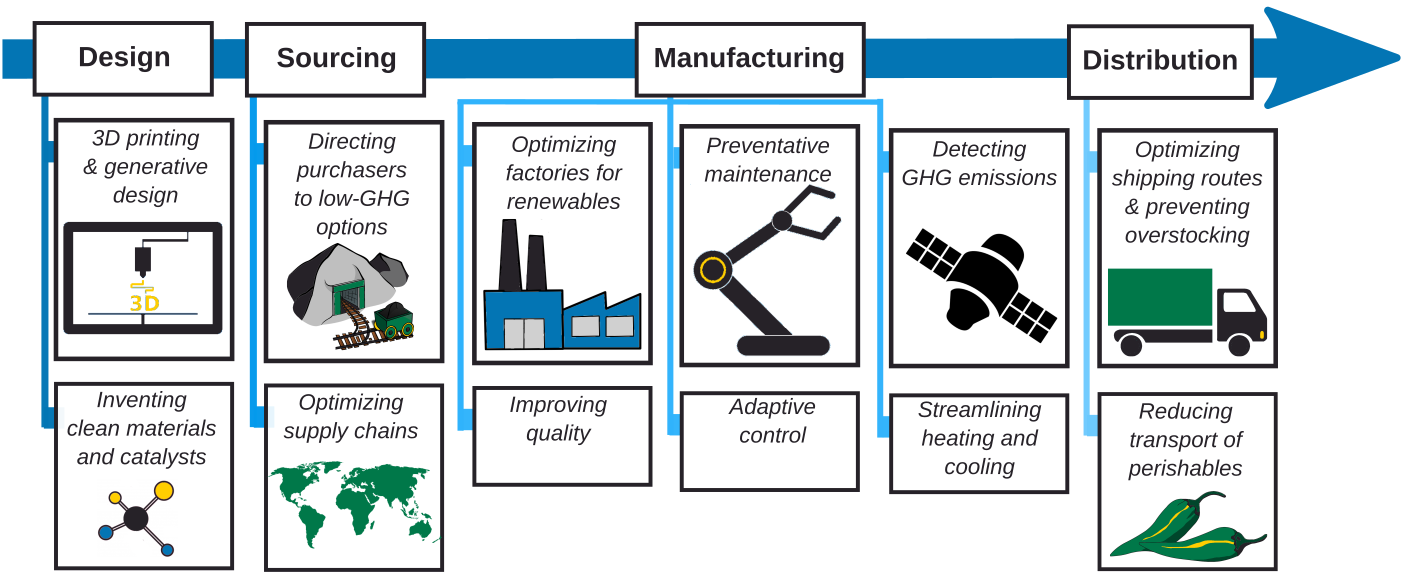
\includegraphics[width=\textwidth]{figures/industry.png}
    \caption{Selected opportunities to use machine learning to reduce greenhouse gas emissions in industry.}
    \label{fig:industry}
\end{figure}

\subsection{Optimizing supply chains}
\label{sec:supplychains}
In 2006, at least two Scottish seafood firms flew hundreds of metric tons of shrimp from Scotland to China and Thailand for peeling, then back to Scotland for sale -- because they could save on labor costs \cite{Cramb2006}. This indicates the complexity of today's globalized \emph{supply chains}, i.e., the organizational processes and shipping networks that are required to bring a product from producer to final consumer. ML can help reduce emissions in supply chains by intelligently predicting supply and demand, identifying lower-carbon products, and optimizing shipping routes. (For details on shipping and delivery optimization, see \S\ref{sec:transportation}.) However, for many of these applications to reduce emissions, firms' financial incentives must also align with climate change mitigation through carbon pricing or other policy mechanisms.

\paragraph*{Reducing overproduction} \Gap \HighRisk\mbox{}\\\label{sec:reducingexcess}The production, shipment, and climate-controlled warehousing of excess products is a major source of industrial GHG emissions, particularly for time-dependent goods such as perishable food or retail goods that quickly fall out of fashion \cite{wang2016energy}. 
Global excess inventory in 2011 amounted to about \$8 trillion worth of goods, according to the Council of Supply Chain Management Professionals \cite{winston2011}. This excess may be in part due to mis-estimation of demand, as the same organization noted that corporate sales estimates diverged from actual sales by an average of 40\% \cite{winston2011}. ML may be able to mitigate these issues of overproducing and/or overstocking goods by improving demand forecasting \cite{akyuz2017ensemble, tsoumakas2019survey}. For example, the clothing industry sells an average of only 60\% of its wares at full price, but some brands can sell up to 85\% due to just-in-time manufacturing and clever intelligence networks \cite{SCMGlobe2016}. As online shopping and just-in-time manufacturing become more prevalent and websites offer more product types than physical storefronts, better demand forecasts will be needed on a regional level to efficiently distribute inventory without letting unwanted goods travel long distances only to languish in warehouses \cite{rizet2010ghg}. Nonetheless, negative side effects can be significant depending on the type of product and regional characteristics; just-in-time manufacturing and online shopping are often responsible for smaller and faster shipments of goods, mostly on road, that lack the energy efficiency of freight aggregation and slower shipping methods such as rail \cite{ugarte2016lean, rizet2010ghg}.

\paragraph*{Recommender systems}\Gap \mbox{}\\\label{sec:recommendersystems}Recommender systems can potentially direct consumers and purchasing firms toward climate-friendly options, as long as one can obtain information about GHG emissions throughout the entire life-cycle of some product. The challenge here lies in hunting down usable data on every relevant material and production process from metal ore extraction through production, shipping, and eventual use and disposal of a product \cite{Hawkins2013,rebitzer2004life}. One must also convince companies to share proprietary data to help other firms learn from best practices. If these datasets can be acquired, ML algorithms could hypothetically assist in identifying the cleanest options.

\paragraph*{Reducing food waste}\Gap \Rec\mbox{}\\\label{sec:foodwaste}Globally, society loses or wastes 1.3 billion metric tons of food each year, which translates to \emph{one-third} of all food produced for human consumption \cite{faofood}. In developing countries, 40\% of food waste occurs between harvest and processing or retail, while over 40\% of food waste in industrialized nations occurs at the end of supply chains, in retail outlets, restaurants, and consumers' homes \cite{faofood}. ML can help reduce food waste by optimizing delivery routes and improving demand forecasting at the point of sale (see \S\ref{sec:supplychains}), as well as improving refrigeration systems \cite{meneghetti2015greening} (see \S\ref{sec:adaptivecontrol}). ML can also potentially assist with other issues related to food waste, such as helping develop sensors to identify when produce is about to spoil, so it can be sold quickly or removed from a storage crate before it ruins the rest of the shipment \cite{fuertes2016intelligent}.

\subsection{Improving materials}
\label{sec:materialsandconstruction}

\paragraph*{Climate-friendly construction}\Gap \Rec\Longterm\mbox{}\\\label{sec:construction}Cement and steel production together account for over 10\% of all global GHG emissions \cite{fischedick2014industry}; the cement industry alone emits more GHGs than every country except the US and China \cite{lehne2018making}. ML can help minimize these emissions by reducing the need for carbon-intensive materials, by transforming industrial processes to run on low-carbon energy, and even by redesigning the chemistry of structural materials. To reduce the use of cement and steel, researchers have combined ML with generative design to develop structural products that require less raw material, thus reducing the resulting GHG emissions \cite{kazi2017dreamsketch}. Novel manufacturing techniques such as 3D printing allow for the production of unusual shapes that use less material but may be impossible to produce through traditional metal-casting or poured concrete; ML and finite element modeling have been used to simulate the physical processes of 3D printing in order to improve the quality of finished products \cite{baturynska}.

Assuming future advances in materials science, ML research could potentially draw upon open databases such as the Materials Project \cite{jain2013commentary} and the UCI Machine Learning Repository \cite{ge2019accelerated} to invent new, climate-friendly materials \cite{ward2016general}. Using semi-supervised generative models and concrete compression data, for example, Ge et al.~proposed novel, low-emission concrete formulas that could satisfy desired structural characteristics \cite{ge2019accelerated}.

\paragraph*{Climate-friendly chemicals}\Gap \Rec\Longterm\mbox{}\\\label{sec:chemicals}Researchers are also experimenting with supervised learning and thermal imaging systems to rapidly identify promising catalysts and chemical reactions \cite{rizkin2019, coley2019graph}, as described in \S\ref{sec:electricity-materials}. Firms are unlikely to adopt new materials or change existing practices without financial incentives, so widespread adoption might require subsidies for low-carbon alternatives or penalties for high GHG emissions.

Ammonia production for fertilizer use relies upon natural gas to heat up and catalyze the reaction, and accounts for around 2\% of global energy consumption \cite{montoya2015challenge}. To develop cleaner ammonia, chemists may be able to invent electrochemical strategies for lower-temperature ammonia production \cite{montoya2015challenge, wood2004review}. Given the potential of ML for predicting chemical reactions \cite{coley2019graph}, ML may also be able to help with the discovery of new materials for electrocatalysts and/or proton conductors to facilitate ammonia production.

\subsection{Production and energy}
\label{sec:demandresponse}
ML can potentially assist in reducing overall electricity consumption; streamlining factories' heating, ventilation, and air conditioning (HVAC) systems; and redesigning some types of industrial processes to run on low-carbon energy instead of coal, oil, or gas. Again, the higher the incentives for reducing carbon emissions, the more likely that firms will optimize for low-carbon energy use. New factory equipment can be very expensive to purchase and set up, so firms' cost-benefit calculations may dissuade them from retrofitting existing factories to run using low-carbon electricity or to save a few kilowatts \cite{gillingham2018cost, plambeck2012reducing, tao2010innovation}. Given the heterogeneity across industrial sectors and the secrecy of industrial data, firms will also need to tailor the requisite sensors and data analysis systems to their individual processes. ML will become a much more viable option for industry when factory workers can identify, develop, implement, and monitor their own solutions internally instead of relying upon outside experts \cite{helper2019profits}. The ML community can assist by building accessible, customizable industry tools tailored for people without a strong background in data science. 

\paragraph*{Adaptive control}\Gap \Rec\mbox{}\\\label{sec:adaptivecontrol}On the production side, ML can potentially improve the efficiency of HVAC systems and other industrial control mechanisms---given necessary data about all relevant processes. To reduce GHG emissions from HVAC systems, researchers have suggested combining optimization-based control algorithms with ML techniques such as image recognition, regression trees, and time delay neural networks \cite{aftab2017automatic, DRGONA2018199} (see also \ref{sec:bldgopt}). DeepMind has used reinforcement learning to optimize cooling centers for Google's internal servers by predicting and optimizing the \emph{power usage effectiveness (PUE)}, thus lowering HFC emissions and reducing cooling costs \cite{evans2016deepmind, gao2014}. Deep neural networks could also be used for adaptive control in a variety of industrial networking applications \cite{ahmed2016green}, enabling energy savings through self-learning about devices' surroundings.

\paragraph*{Predictive maintenance} \Gap\mbox{}\\\label{sec:predictive}ML could also contribute to predictive maintenance by more accurately modelling the wear and tear of machinery that is currently in use, and interpretable ML could assist factory owners in developing a better understanding of how best to minimize GHG emissions for specific equipment and processes. For example, creating a \emph{digital twin} model of some industrial equipment or process could enable a manufacturer to identify and prevent undesirable scenarios, as well as virtually test out a new piece of code before uploading it to the actual factory floor -- thus potentially increasing the GHG efficiency of industrial processes \cite{Glaessgen2012, Tao2018}. Digital twins can also reduce production waste by identifying broken or about-to-break machines before the actual factory equipment starts producing damaged products. Industrial systems can employ similar models to predict which pipes are liable to spring leaks, in order to minimize the direct release of GHGs such as HFCs and natural gas.


\paragraph*{Using cleaner electricity}\Gap \Rec\mbox{}\\\label{sec:electritydemand}ML may be particularly useful for enabling more flexible operation of industrial electrical loads, through optimizing a firm's \emph{demand response} to electricity prices as addressed in \S\ref{sec:electricity-systems}. Such optimization can contribute to cutting GHG emissions as long as firms have a financial incentive to optimize for minimal emissions, maximal low-carbon energy, or minimum overall power usage. Demand response optimization algorithms can help firms adjust the timing of energy-intensive processes such as cement crushing \cite{Zhang2016} and powder-coating \cite{Rockwell} to take advantage of electricity price fluctuations, although published work on the topic has to date used relatively little ML. Online algorithms for optimizing demand response can reduce overall power usage for computer servers by dynamically shifting the internet traffic load of data providers to underutilized servers, although most of this research, again, has focused on minimizing costs rather than GHG emissions \cite{buchbinder2011online, Horner2016}. Berral et al.~proposed a framework that demonstrates how such optimization algorithms might be combined with RL, digitized controls, and feedback systems to enable the autonomous control of industrial processes \cite{Berral2010}.

\subsection{Discussion}
\label{sec:industrydiscussion}
Given the globalized nature of international trade and the urgency of climate change, decarbonizing the industrial sector must become a key priority for both policy makers and factory owners worldwide.  As we have seen, there are a number of highly impactful applications where ML can help reduce GHG emissions in industry, with several caveats. First, incentives for cleaner production and distribution are not always aligned with reduced costs, though policies can play a role in aligning these incentives. Second, despite the proliferation of industrial data, much of the information is proprietary, low-quality, or very specific to individual machines or processes; practitioners estimate that 60-70\% of industrial data goes unused \cite{Coffey2019, Gualtieri2016}. Before investing in extensive ML research, researchers should be sure that they will be able to eventually access and clean any data needed for their algorithms. Finally, misjudgments can be very costly for manufacturers and retailers, leading most managers to adopt risk-averse strategies towards relatively untested technologies such as ML \cite{helper2019profits}. For this reason, ML algorithms that determine industrial activities should be robust enough to guarantee both performance and safety, along with providing both interpretable and reproducible results \cite{henderson2018deep}.
\end{document}